
\documentclass[journal,a4paper,12pt]{IEEEtran}

\usepackage{graphicx}
\usepackage{tikz}
\usepackage[margin=1in]{geometry}
\usepackage[most]{tcolorbox}
\usepackage{chessboard}
\usepackage{float}
\usepackage{hyperref}
\usepackage{url}
%\usepackage{biblatex}
\usepackage{cite}
\usepackage{setspace}
\usepackage{subfigure}

%
% If IEEEtran.cls has not been installed into the LaTeX system files,
% manually specify the path to it like:
% \documentclass[journal]{../sty/IEEEtran}

% correct bad hyphenation here
\hyphenation{op-tical net-works semi-conduc-tor}



\doublespacing
\begin{document}
%
% paper title
% can use linebreaks \\ within to get better formatting as desired
\title{Towards Differential Drag Control for\\ Autonomous Multiagent Satellites in\\ Kerbal Space Program}

\author{
\textbf{Caleb Ashmore Adams}\\
\textit{Department of Computer Science}, University of Georgia\\
\textit{Small Satellite Research Laboratory}, University of Georgia\\
1510 Cedar St. Athens, GA 30602\\
% 770-314-8422\\
pieninja@uga.edu
}


% The paper headers
\markboth{UGA CSCI/ARTI 6550 Term Project}%
{Shell \MakeLowercase{\textit{et al.}}: The Title of your Paper}
% The only time the second header will appear is for the odd numbered pages
% after the title page when using the twoside option.
%

% make the title area
\maketitle

% The Abstract
\begin{abstract}
  The concept of differential drag has received a significant amount of research
  attention due to its relevance with emerging space technologies and its potential
  use in satellite swarms \cite{horsley}. Furthermore, the computational complexity
  of many differential drag based satellite swarms makes them ideal for automation
  through Artificial Intelligence (AI) \cite{swarm_ai}. However, this computational
  complexity - coupled with the necessity for high fidelity physics simulations -
  quickly becomes a long and arduous challenge filled with various optimization
  problems \cite{sin}. Due to the intended brevity of this research, simpler models
  are preferable. Humorously, this makes the popular aerospace engineering simulation
  game, Kerbal Space Program (KSP), an ideal candidate due to simplicity and
  customizability (mods). AI does, after all, have a wonderful history of being
  applied to video games for the aforementioned reasons \cite{ai_games_book}\cite{wiki_ai_games}.
  Thus, this project seeks to implement autonomous rendezvous
  in KSP using mods, Python, and C\#. This research will roughly follow
  Russell and Norvig’s Planning and Moving (chapter  25.4, 25.5, and 25.6) and Multiagent
  Planning (chapter 11.4) \cite{class_book}.

\end{abstract}

\IEEEpeerreviewmaketitle


% ==============================================================================
%
% section
%
% ==============================================================================
\section{Introduction}

The source code for this project, which is referenced within this document, is located
within a public repository
at: https://github.com/piepieninja/KSP-DiffDrag. The requirements to run the software
is listed in a \texttt{README.md} file in the root of the repository. In general,
the repository seeks to be as self-explanatory as possible.

% =====================================
% subsection
% =====================================
\subsection{Project Structure}
The project is managed via a git repository located at the aforementioned link.
Inside the \texttt{src} folder is where most of the code is. There is a \texttt{src/kos}
folder which contains all of the kerbalscript, an \texttt{src/example} folder which includes
several videos and python examples, and \texttt{src/DragDetector} folder which contains
the code relating lower-level game mods. This folder is one of several microsoft
visual studio projects. Other folders or scripts within the \texttt{src}
folder are either previous tests that I often reference, or features in progress that are
not relevant to this immediate research.
The \texttt{util} folder contains several bash scripts which are used to manage the state
of the game so that I can have a constant set of start states. These scripts were useful for
my workflow during this project and contain little substance relating to this research.
Furthermore, the utility scripts typically load save states from the \texttt{data} folder
into the game pre-launch, but also load kerbalscript into the game from the \texttt{src/kos}
folder. The \texttt{docs} folder is where all latex is located and the \texttt{bin} folder
is used to store binary releases of custom mods, these are untracked by git and will not
show up in the repository.

% =====================================
% subsection
% =====================================
\subsection{differential drag}
Put simply, drag is a force that acts opposite to the relative motion of any object
moving with respect to a surrounding fluid \cite{drag_deff}. For the purposes of this
research I will attempt to simplify our interpretation of drag as much as possible.
The drag equation is as follows:
\begin{equation}
F_D = \frac{1}{2} \rho u_a^2 C_D A
\end{equation}
In formula $1$, the drag equation, $F_D$ is the force of drag acting on the object.
$\rho$ is the mass density of the fluid the object moves through and $u$ is the relative
velocity of the fluid immediately surrounding the object. $C_D$ is the coefficient of
drag of the object and $A$ is the surface area of the object that collides with
particles in the fluid. Low Earth Orbit, in our case Low Kerbin Orbit (LKO),
has a very low $\rho$ value. Interestingly,
the density of the atmosphere at $400km$ is still significant enough to
generate non-negligible drag on spacecraft.

\begin{figure}[h!]
  \centering
  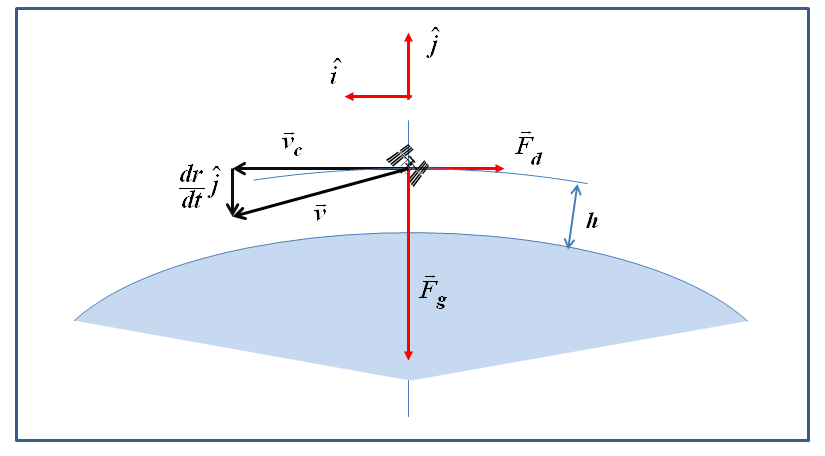
\includegraphics[width=2.5in]{img/ISSpng}
  \caption{The international space station (ISS) shown here being affected by a
  drag force, $F_d$. The gravitational force $F_g$ is also shown, along with the
  ISS's velocity $\frac{dr}{dt}\hat{j}$ and tangential velocity $v_c$ \cite{iss_boi}. }
  \label{drag_detector}
\end{figure}

The term differential drag
comes from the fact that a spacecraft can reorient itself to increase its surface
Area $A$ that is exposed to oncoming particles within the atmosphere. This means that any
spacecraft capable of orienting itself is also capable of generating a maximum
and a minimum amount drag.
The primary motivation for this research was to see if KSP had similar physics and
if I could design a differential drag system within the game. To perform Differential
Drag in KSP it is necessary to calculate
these values in real time to generate the force $F_D$.
\begin{equation}
F_L = \frac{1}{2} \rho u_a^2 C_L A
\end{equation}
The lift equation, seen as equation 2, is very similar to drag, but acts as an opposite force. The
coefficient of lift $C_L$ depends on materials. The area $A$ is the amount of surface area contributing
to lift. It is necessary to calculate the lift on an object, as the net
force acting on an object is $F = F_D - F_L$. Thus, there are several cases where lift
can play a significant role in the rendezvous procedures of two spacecraft \cite{lifty_boi}.


% =====================================
% subsection
% =====================================
\subsection{Kerbal Space Program}
Kerbal Space Program (KSP) is a popular video game among space enthusiasts and
engineers. KSP takes a hyper realistic approach towards simulating and gamifying
the process of building and operating spacecraft. KSP takes place within a fictitious
solar system that is nearly identical to ours (with the exception that it is populated
by little green aliens). The Earth-like planet from which all rockets are launched
is known as Kerbin. All of the research within this paper takes place below Low Kerbin
Orbit (LKO), analogous to Low Earth Orbit (LEO), at an altitude of $60000$m to
$70000$m.

\begin{figure}[h!]
  \centering
  \subfigure[The atmospheric pressure and temperature of Kerbin by altitude \cite{Kerbal_wiki}.]{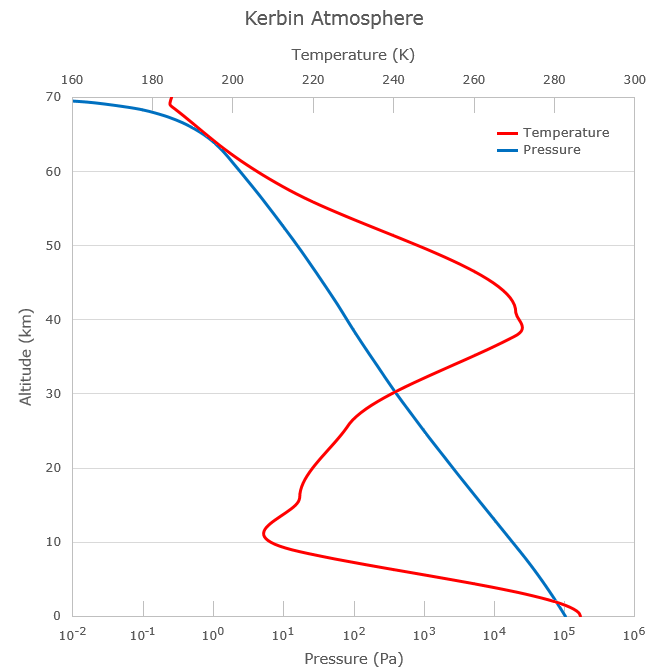
\includegraphics[width=2.5in]{img/KerbinAtmosphereTP}}
  \subfigure[The atmospheric density of Kerbin by altitude \cite{Kerbal_wiki}.]{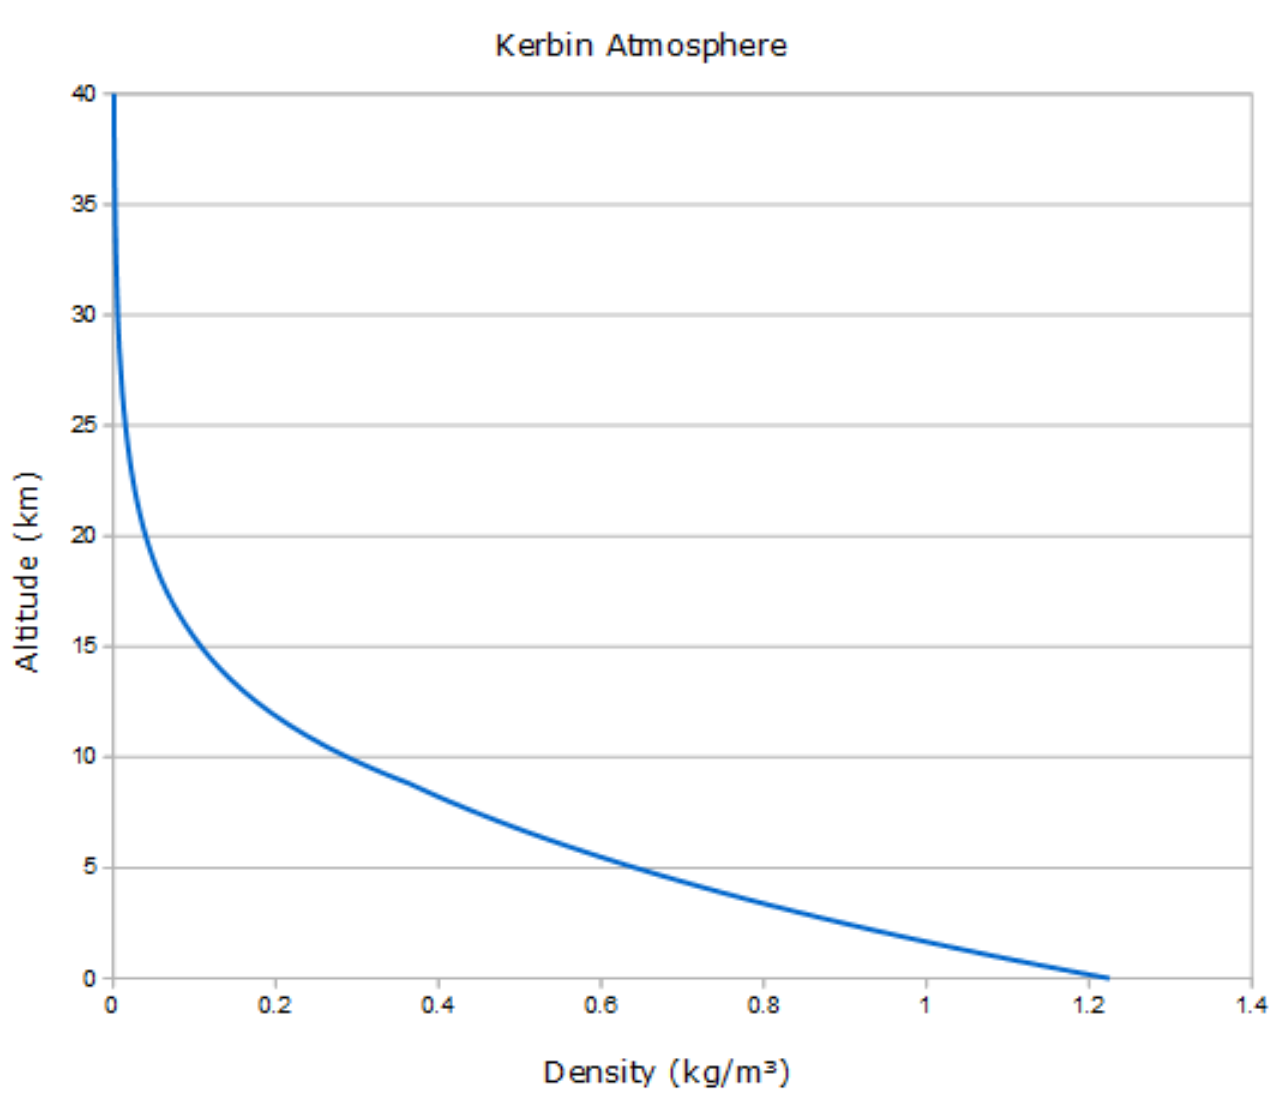
\includegraphics[width=2.5in]{img/KerbinFUQ}}
  % \caption{Simulation results for the network.}
  \caption{Critical measurements of the Kerbin atmosphere related to altitude}
  \label{Kerbin_atmo}
\end{figure}

As explained in the differential drag section, the presence of a fluid (in our case
an atmosphere) is necessary to perform differential drag. The typical KSP player
would recommend avoiding going below
$70000$m, as this will cause drag due to the atmosphere. However, this is exactly what
is desired. It has been reported several times on the forums that there are no
atmospheric effects above $70000$m. I have, however, identified some small effects
if the Drag Detector (mentioned in the Modding KSP section) is enabled while climbing.
Future studies may further investigate this phenomenon.

In addition to a hyper-realistic atmosphere, KSP also emulates the engineering requirements
of spacecraft. This means that spacecraft must satisfy various power, thermal, data,
or communication constraints. It is fairly simple to design around these specifications and
often ends up boiling down to restrictions such as: \textit{will my spacecraft generate more power from its
solar panels than it uses to run}? Overall, a balanced design is needed to have a well
functioning spacecraft.

% =====================================
% subsection
% =====================================
\subsection{Modding Kerbal Space Program and\\ Craft Design}
KSP has a large community of modders who edit source code or use the KSP
C\# Application Programming Interface (API) to create new and interesting content.
In order to get the multiagent functionality required for this research, the
Kerbal Operating System (KOS) mod was used \cite{kos}. The KOS mod provides several
in-game computers that are capable of running a custom scripting language known
as kerbalscript. Approximately half of this research is written in kerbalscript.
KOS and kerbalscript are accessible
over a local area network (LAN) via telnet
protocol. Often this feature was used to run multiple programs on a craft as once.

\begin{figure}[h!]
  \centering
  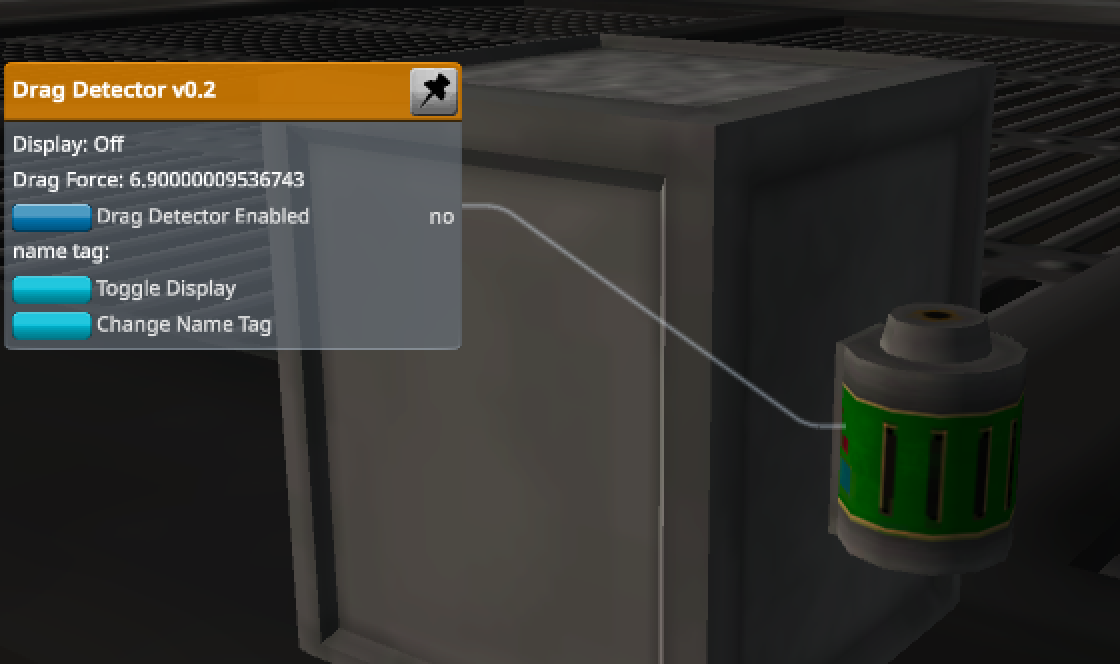
\includegraphics[width=2.5in]{img/dragdetector}
  \caption{The Drag Detector, in green seen on the right, interfaced to a simple cube frame.}
  \label{drag_detector}
\end{figure}

The other half of this research is written in C\#. This is due to the fact that
KOS and kerbalscript do not grant access to some of the lower level physics that are required
to perform accurate differential drag maneuvers. I have many hours of reading through very
dry forum posts to thank for that knowledge.
After researching the drag physics of KSP, it was clear to me that I was going to
need to modify the game so that I could have access to lower level physics. Due to
this limitation a custom part was created, dubbed the \textit{Drag Detector}. The
Detector can be placed on any spacecraft.

Thankfully, the game makes some simplifying assumptions and not all parts are guaranteed to
generate drag or lift. Additionally, the game does not calculate drag along a part's
real surface area. The game generates \textit{drag cubes} to approximate the drag
effects of drag on a given part \cite{ksp_api}.
The Drag Detector works by iterating through
parts and components on a spacecraft to sum the total drag force acting on a craft.
For each drag vector on a part, it finds the magnitude and direction for the force.
It then does this for each component on the craft that contributes to a lift force.
These calculations can be seen in the source code at \texttt{src/DragDetector/\\DragDetector/MyClass.cs}.
The process to calculate this was uncovered by Nathan Kell and is publicly available
on github \cite{aero_gui}.
The Drag Detector finds the net drag force acting on the craft and publishes this to
a variable accessible via KOS and kerbalscript.

\begin{figure}[h!]
  \centering
  \subfigure[The craft seen in a low drag configuration]{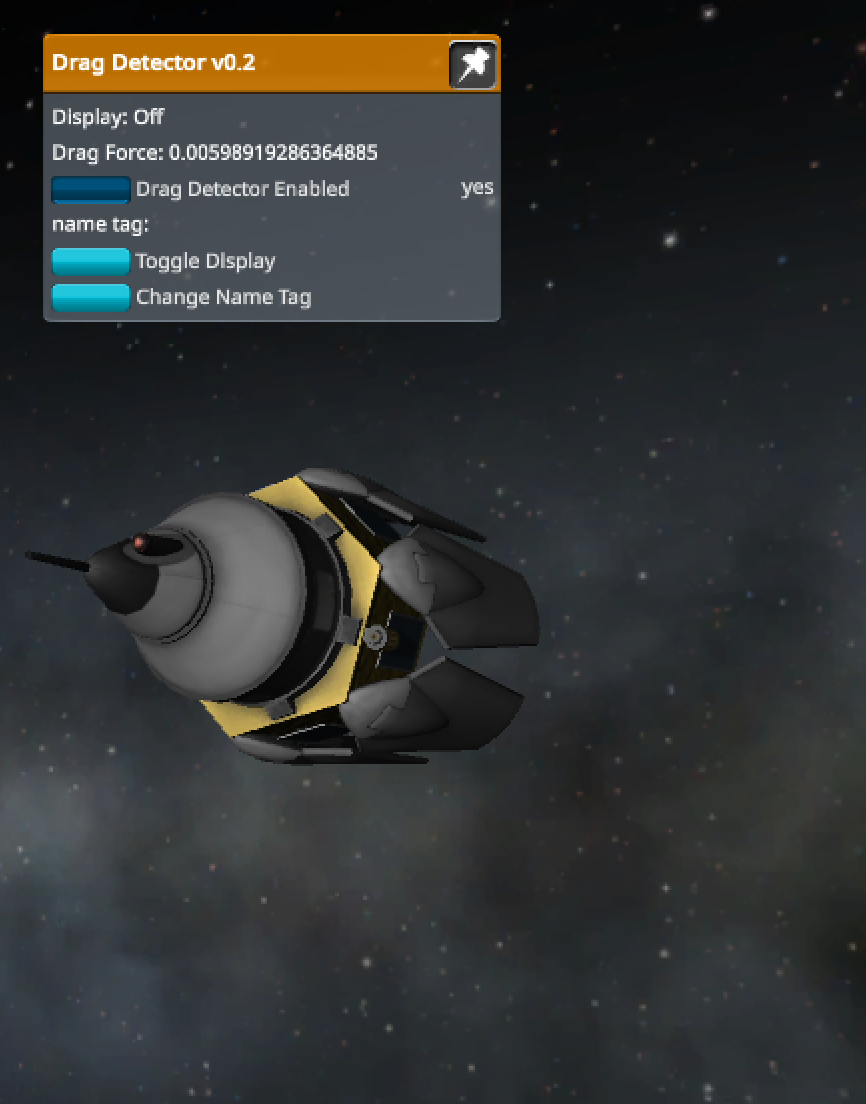
\includegraphics[width=2.5in]{img/boi1}}
  \subfigure[The craft seen in a high drag configuration]{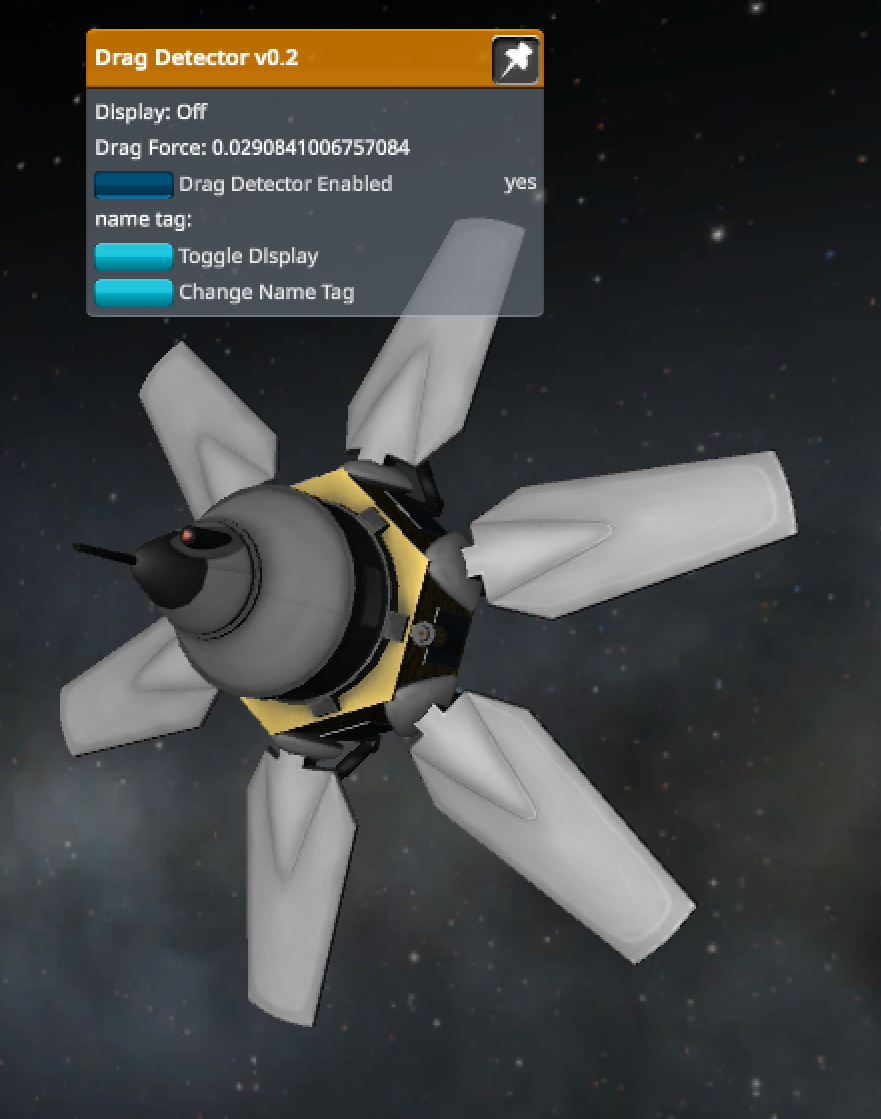
\includegraphics[width=2.5in]{img/boi2}}
  % \caption{Simulation results for the network.}
  \caption{The spacecraft designed to perform differential drag maneuvers in lower LKO.
  Note that at $~69000$m the Drag Detector measures $~0.006$kN of drag force in the low drag configuration
  and $~0.03$kN of drag force in the high drag configuration, a 5x increase in force. }
  \label{Kerbin_sat}
\end{figure}

The spacecraft that I designed can be seen in figure \ref{Kerbin_sat}. The three key
design choices that enabled this craft to operate as desired are the KOS computer,
the custom built Drag Detector, and the six aerobreaks. The KOS computer allows for
the craft to calculate its position, obtain knowledge about the states of other
craft, have knowledge of its own state, and perform maneuvers. The Drag Detector,
as mentioned before, allows the craft's KOS computer to have access to lower level
drag physics. Finally, the six radial aerobreaks allow the craft to increase or
decrease it's surface area to enter or exit high and low drag configurations.

% ==============================================================================
%
% section
%
% ==============================================================================
\section{Multiagent Satellites}

% =====================================
% subsection
% =====================================
\subsection{The Rendezvous Problem}
Lin et al. state that the multiagent rendezvous problem is to devise "local" control
strategies, one for each agent, which without any active communication between agents,
cause all members of the group to eventually rendezvous at a single unspecified location \cite{lin_multi}.
Furthermore, Russell and Norvig describe three particular values that any such multiagent
system is likely to have per agent \cite{class_book}:

\begin{enumerate}
  \item Cohesion, a positive score for getting closer to the average position of the neighbors
  \item Separation, a negative score for getting too close to any one neighbor
  \item Alignment, a positive score for getting closer to the average heading of the neighbors
\end{enumerate}

With the given descriptions, one can easily imagine a purely Cohesion-based rendezvous
system where agents converge to some middle point. If we view a given agent as a
particle $p$ placed randomly within a place, we can use each particle's $(x,y)$
value to calculate a centroid. The unit vector at each particle pointing to the
centroid represents the movement for the particle that results in the most immediate
cohesion.

\begin{equation}
  C(x,y) = (\frac{x_1 + x_2 \hspace{1mm} ... + x_n}{n} , \frac{y_1 + y_2 ... \hspace{1mm} + y_n}{n})
\end{equation}

I have provided an example python program at \texttt{src/examples/scatter\_join.py} that
performs a naive Cohesion-based rendezvous. The program generates 8 points $p$ with and
gives them random $(x,y)$ coordinates from $0.0$ to $20.0$. At each time step each
individual $p$ calculates the global centroid, as defined in equation 3, and
moves a constant unit in that direction. The effect is that all agents converge on
the same location in an orderly way while only controlling themselves and not coordinating
efforts.

\begin{figure}[h!]
  \centering
  \subfigure[Frame 1 in naive Cohesion-based rendezvous, showing a dispersion of particles]{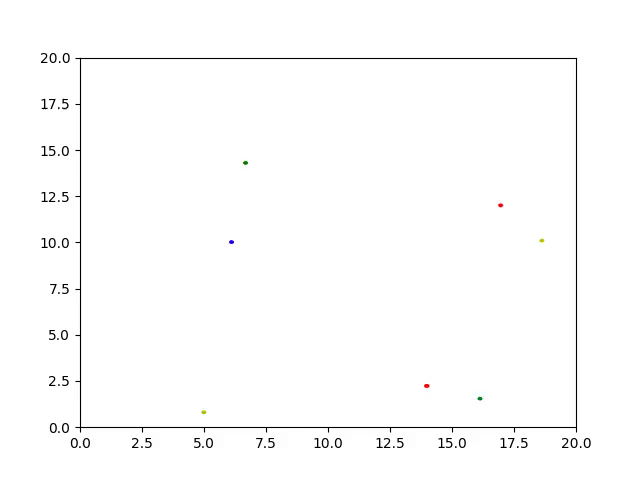
\includegraphics[width=1.25in]{frames/output01}}
  \subfigure[Frame 20 in naive Cohesion-based rendezvous, showing cohesion towards a centroid]{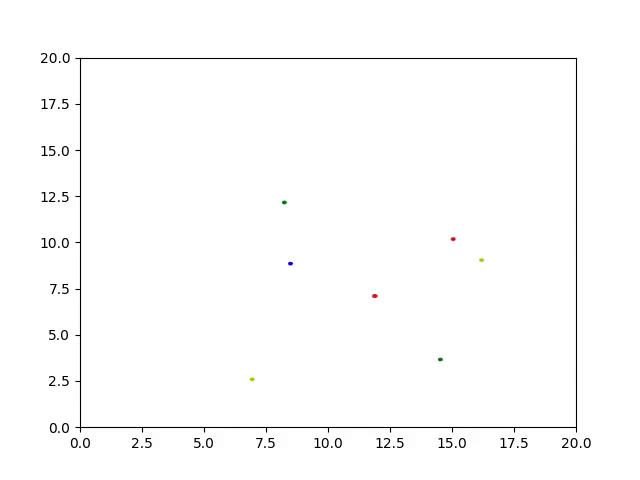
\includegraphics[width=1.25in]{frames/output20}}
  % \caption{Simulation results for the network.}
  \label{rend_set1}
\end{figure}
\begin{figure}[h!]
  \centering
  \subfigure[Frame 40 in naive Cohesion-based rendezvous, showing further cohesion towards a centroid]{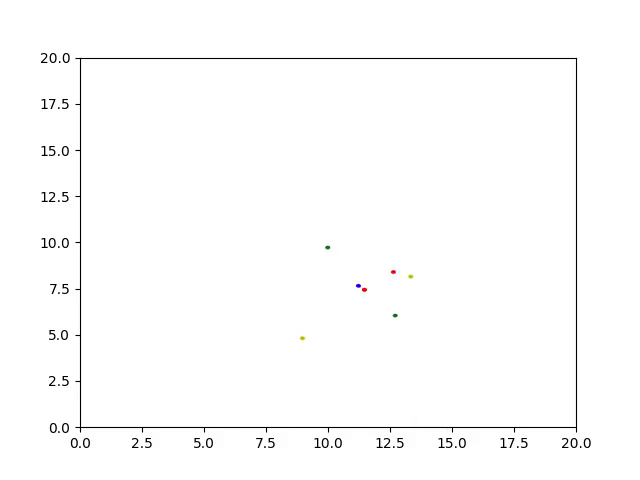
\includegraphics[width=1.25in]{frames/output40}}
  \subfigure[Frame 55 in naive Cohesion-based rendezvous, showing near completion of the objective]{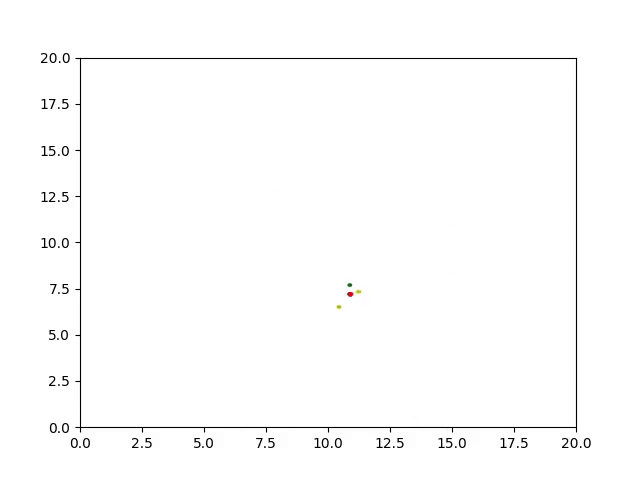
\includegraphics[width=1.25in]{frames/output55}}
  % \caption{Simulation results for the network.}
  \label{rend_set2}
  \caption{For the convenience of the reader, a pre-run example animation of the
  naive Cohesion-based rendezvous is available under \texttt{src/examples/animation.mp4}}
\end{figure}

However, this alone is typically not sufficient. Lin further argues that the typical
agent in a multiagent rendezvous problem has a logical limit on its sensing
capabilities \cite{lin_multi}. To demonstrate a solution to this constraint I have
provided another example program \texttt{src/examples/\\scatter\_join\_limited\_sensing.py}
that contains a sensing radius $r$ outside of which an agent will not be able to detect
another agent. The setup is nearly identical to the naive Cohesion-based rendezvous
mentioned before. The only difference is that each agent calculates a local centroid
that only consists of the agents within the sensing radius $r$. Furthermore, for the
convenience of the reader, a pre-run example animation of the sense-limited Cohesion-based
rendezvous is available under \texttt{src/examples/animation2.mp4}. This implementation does
produce local regions of centroids as a consequence. This means that a sensing-limited
solution such as this is not guaranteed to yield a solution. A possible way to resolve
this is to allow clumped agents to perform a random walk within the known sensing
radii of their neighbors. If we view the state space as the set of floats that could
represent the locations of the agents and, if the state space is finite, then this may solve
the issue. However, if the state space is infinite then there is no guarantee two
agents outside of each others sensing radii will rendezvous. Thus, to simplify the
problem within this research I will not assume sensing-limited agents.

\begin{figure}[h!]
  \centering
  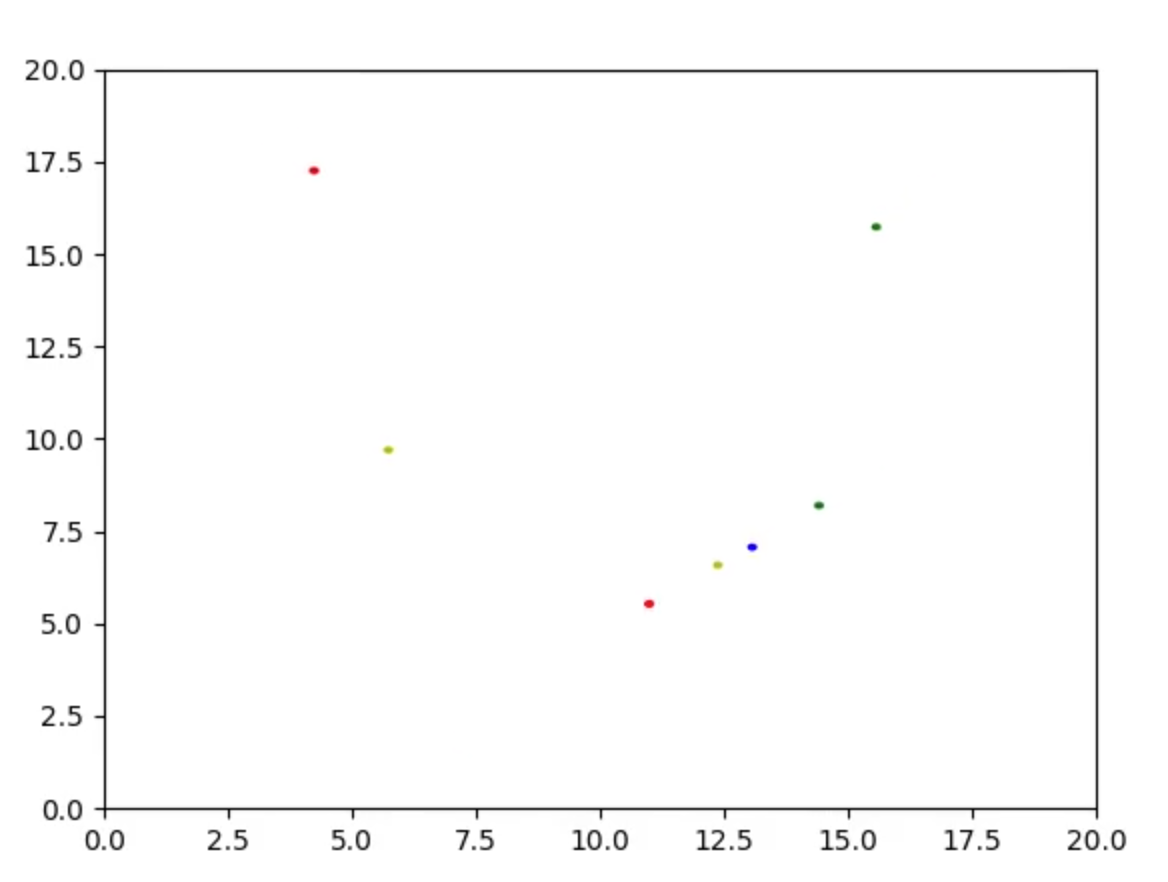
\includegraphics[width=2.5in]{img/yeetset1}
  \caption{An example of local clustering with sense-limited Cohesion-based rendezvous}
  \label{yeet_set1}
\end{figure}


% =====================================
% subsection
% =====================================
\subsection{The Real Rendezvous Problem}
The real rendezvous problem refers to the fact that this multiagent rendezvous must
occur in a space environment. There are a few key factors to consider when performing
a traditional rendezvous in orbit \cite{auto_rend}. Some of such factors include relative speed
from the agent to the target, acceleration due to gravity in the moment, relative orientation
of the crafts, and signal delay between the craft.
A key concept relating to the orbital rendezvous problem is the concept of orbital
maneuvers, the most important of which is the phasing maneuvers. A phasing maneuver, in our
simple case, changes a craft's velocity so that it enters a different orbit. A phasing
orbit allows a craft to move closer to another in preparation to synchronize orbits.
The simplest use of a phasing orbit to rendezvous with another craft is its use
in a Hohmann transfer \cite{okwow}.

\begin{figure}[h!]
  \centering
  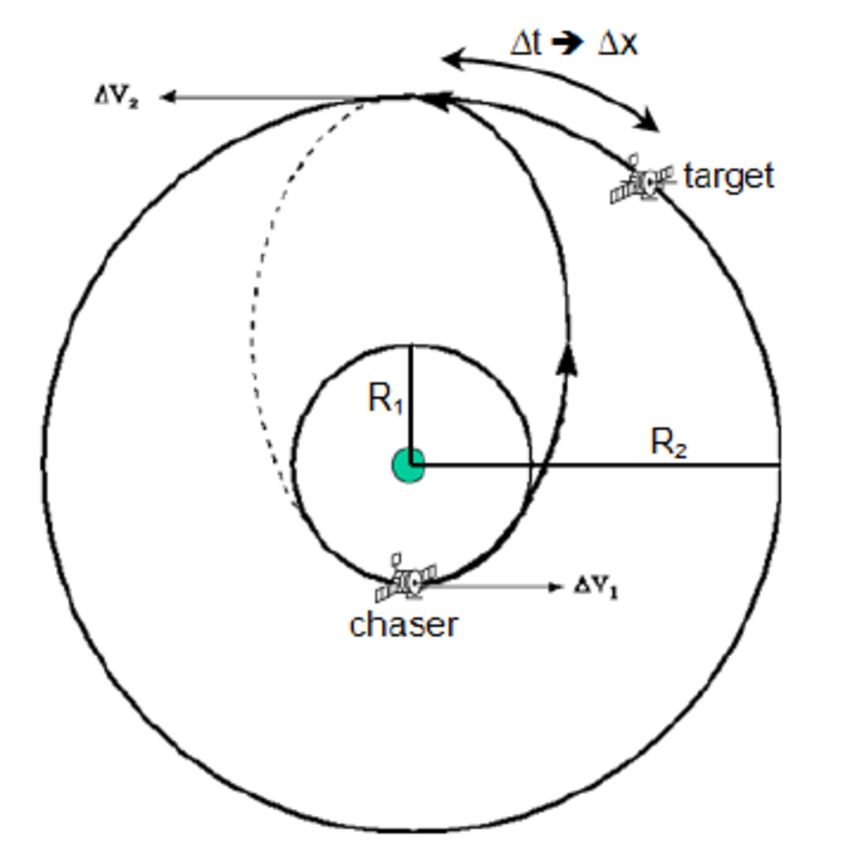
\includegraphics[width=2.5in]{img/HohmannTransfer}
  \caption{A simple Hohmann transfer showing a the distinction between the chasing
  satellite and the target satellite}
  \label{hohmann}
\end{figure}

\subsection{Current Solutions}
In order for a set of maneuvers, such as the Hohmann transfer, to be executed, a
change in velocity is required. Imagine, for a moment, that the chasing and target
satellites in figure \ref{hohmann} were reversed. It is still possible for the satellite
to drop to a lower orbit via a Hohmann transfer. Notice, this is the only way Differential
Drag reliant spacecraft could perform a rendezvous \cite{horsley}.

Essentially, when constrained to any two given satellites the differential drag
technique is to have the trailing satellite become the chaser and the leading
satellite become the target. The chaser goes into a high drag configuration to
drop its orbit and move more quickly towards the target. Approximately half way
to the target, the target and chaser switch drag configurations to roughly align
their orbits again. When the drag maneuvers are over, both craft return to their
low drag configurations \cite{sanny}.

\begin{figure}[h!]
  \centering
  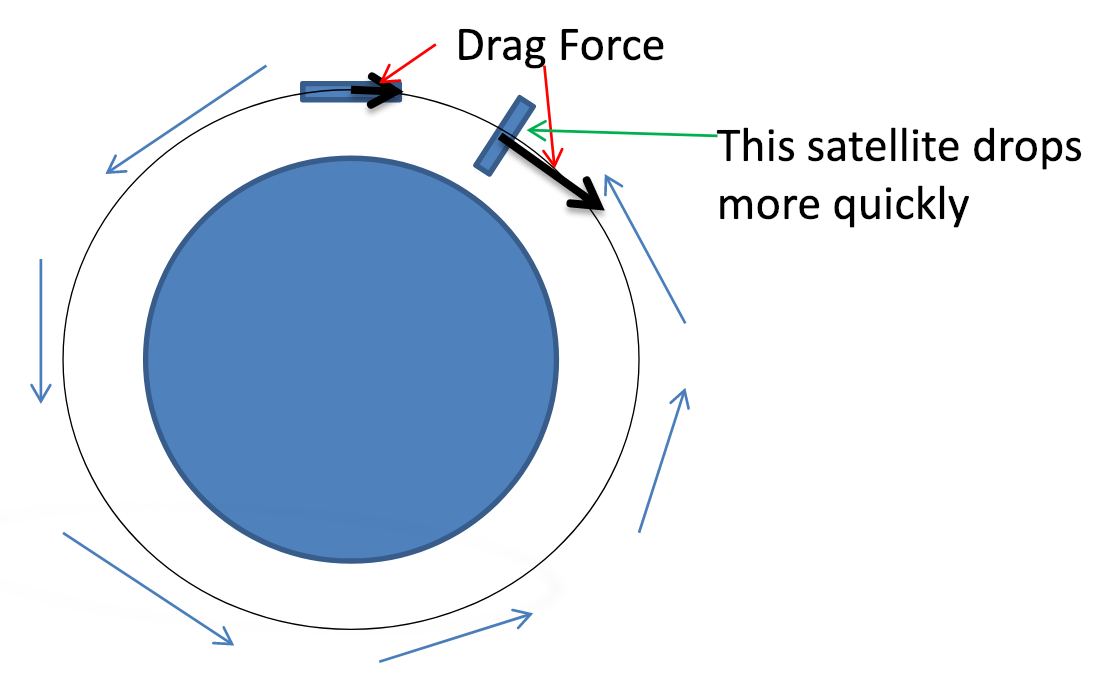
\includegraphics[width=2.5in]{img/ayee1}
  % \caption{A simple Hohmann transfer showing a the distinction between the chasing
  % satellite and the target satellite}
  % \label{hohmann}
  \caption{The trailing satellite, the chaser, goes into a high drag configuration.
  The target maintain a low drag configuration.}
\end{figure}
\begin{figure}[h!]
  \centering
  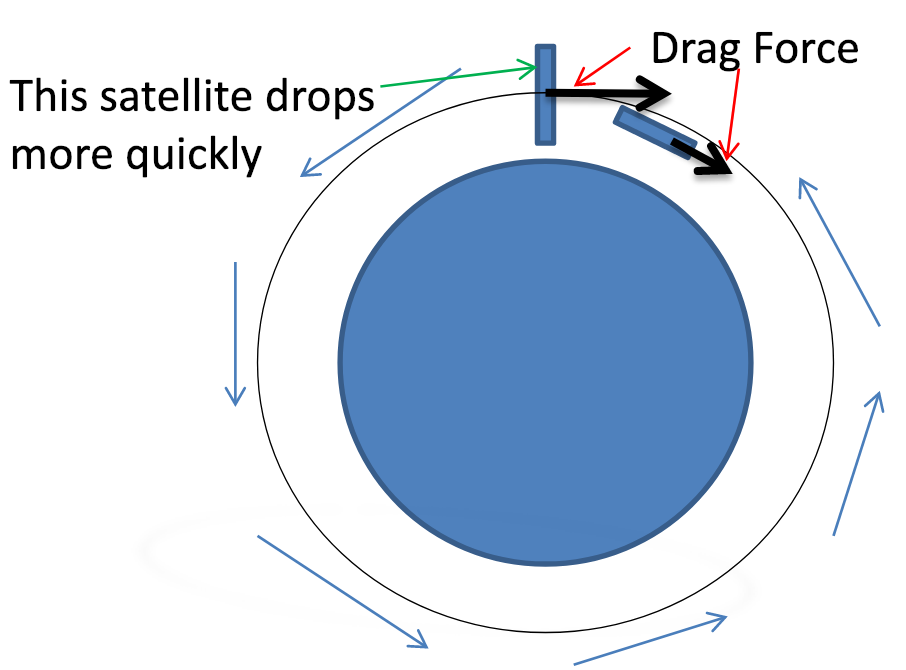
\includegraphics[width=2.5in]{img/ayee2}
  % \caption{A simple Hohmann transfer showing a the distinction between the chasing
  % satellite and the target satellite}
  % \label{hohmann}
  \caption{The trailing satellite, the target, switches into a high drag configuration.
  The chaser switches to a low drag configuration.}
\end{figure}
\begin{figure}[h!]
  \centering
  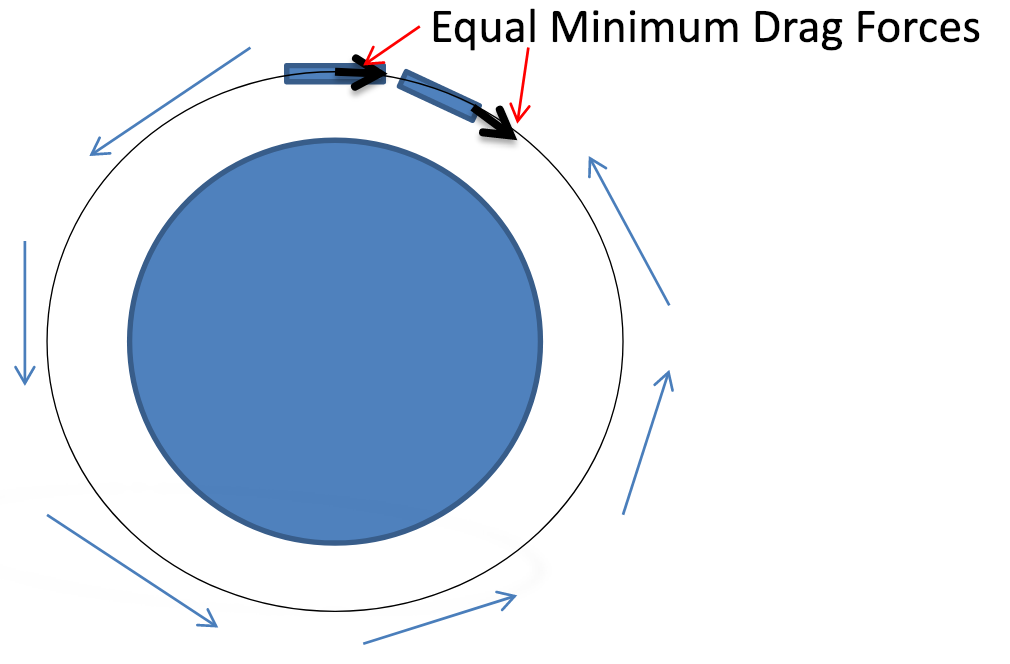
\includegraphics[width=2.5in]{img/ayee3}
  \caption{Both satellites are in a low drag configuration and the distance between
  them has decreased.}
  \label{oof}
\end{figure}

This technique also extends to large fleets of craft. Planet Labs, a company that operates
large fleets of small spacecraft, utilizes similar drag control to maintain flight formations
utilizing restrictions such as cohesion, separation, alignment mentioned by Russell and Norvig.
Similarly, they utilize phasing orbits and the available ratio of low-drag to
high-drag ballistic coefficients of the satellites. As recently as 2016 they have shown
success in using such techniques to maintain an ordered multiagent group of 12 satellites \cite{planet_lab}.

Some differential drag and lift designs assume that the satellite has a retractable
or manipulable surface to be used for diverting fluid flow \cite{lift_drag}.
This is where I got my idea to use retractable aerobreaks, similar to how
planes utilize wing flaps. Additionally, current state of the art multiagent satellite
control algorithms assume a distributed and centralized system where individual
agents choose actions based on limited information \cite{dist_boi}. This
aligns well with Russell and Norvig's definition of multiagent planning. Additionally,
such systems typically account for more forces than simply drag and lift, so this
makes the potential for rendezvous and formation flight more promising \cite{dist_boi}.

% ==============================================================================
%
% section
%
% ==============================================================================
\section{Analysis}

% =====================================
% subsection
% =====================================
\subsection{Functional Rendezvous}
Firstly, an ability to enter and exit minimum and maximum drag configurations was
successfully developed. The satellites are also able to characterize their drag
environments accurate to the game's physics, with an earlier example showing that
the high-drag configuration was 5x that of the low drag configuration. Additionally,
a method for easily calculating drag was modified into the game.

\begin{figure}[h!]
  \centering
  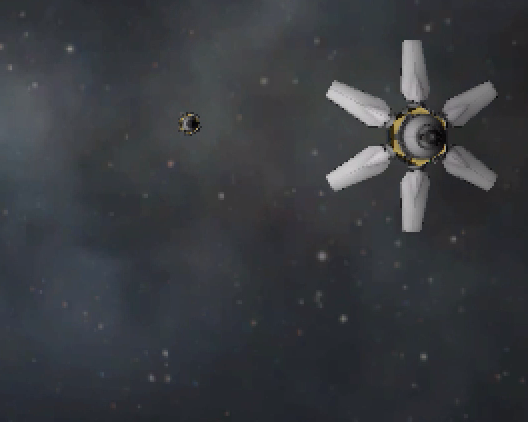
\includegraphics[width=2.5in]{img/draggy}
  \caption{Moments after the leading satellite switches from a low drag configuration
  to a high drag configuration to attempt to phase with the other satellite.}
  \label{drag}
\end{figure}

I was able to successfully demonstrate a two-system rendezvous in KSP utilizing
the systems mentioned above, though there are many problems. For the convenience of the
reader I have some sample videos in the \texttt{src/examples} folder that show
relative rendezvous. An example of an early test that generated a close approach
can be seen in the \texttt{a\_test\_21.mov} video. The test was from an early
successful test where the closest approach of the two satellites was approximately
$85$ meters. Later tests, such as the as \texttt{phase\_swap.mov} demonstrates the
alternating phases of high-drag and low-drag maneuvers swapping close to the final
rendezvous approach of the two satellites. The separation distance in this case
reaches less than $6$ meters, a significant improvement upon earlier tests. The
startup sequence to initiate the program is shown in \texttt{startup\_example.mov}.
As shown, it is necessary to synchronize the scripts before running. The KOS shells
then run the scripts that allow the satellites to rendezvous.



% % =====================================
% % subsection
% % =====================================
% \subsection{Issues with KSP Drag}
% asdf

% =====================================
% subsection
% =====================================
\subsection{Conclusion}
Overall, This research presented more problems and unanswered questions than it did solutions.
I mentioned at the start of this paper that traditional simulation methods present a
"long and arduous challenge". This has been no different.
Obtaining the background knowledge needed to accomplish this research was quite
time consuming. Many hours debugging, web crawling, and documentation hunting
was required to have enough information about the systems being used to make significant
progress towards solving any multiagent problem. Much of what is
discussed or implemented here I learned exclusively for this research. My initial
view that KSP would be simple to modify was very wrong. In order to modify KSP for
the desires of this project one must be nearly-familiar with amature full stack
game development. For this research I learned two new programming languages, information
about 3D modeling, Unity, and spent more than
40+ hours debugging obscure game engine related errors outside of simply implementing
the multiagent portion of this research. It is for this reason (knowing that it would be hard for others to
run my exact programs) that I have included videos of the program's operating as well
as simplified python scripts to demonstrate the fundamental concepts.

\begin{figure}[h!]
  \centering
  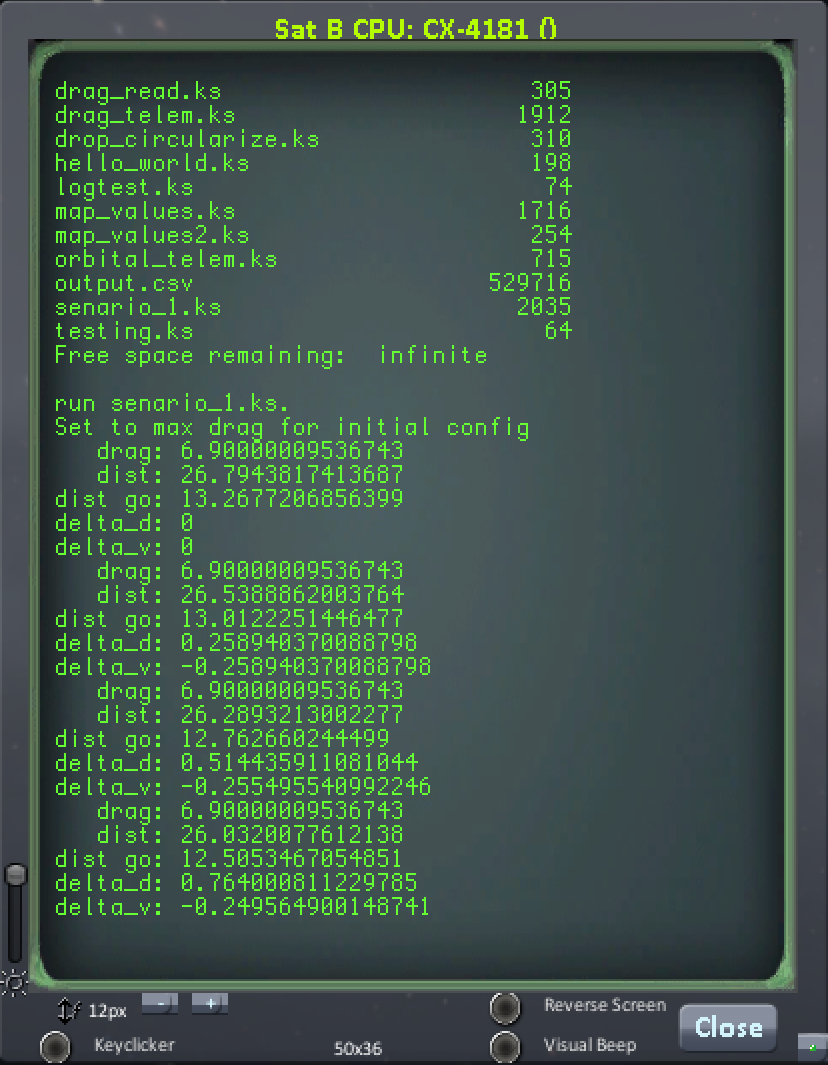
\includegraphics[width=2.5in]{img/kosterm}
  \caption{An example of a KOS terminal operating the \texttt{senario\_1.ks} program,
  which performs the rendezvous. The detected drag, labeled \texttt{drag}, and the
  target separation distance, labeled \texttt{dist}, are shown along with other telemetry.}
  \label{kos}
\end{figure}

Cohesion-based rendezvous methods have proven ineffective for the
multiagent systems I have been testing. I realized fairly quickly that Cohesion-based
methods can be viewed as "greedy". Such a system often chooses to lower an orbit
too quickly, getting much closer to the target satellite, at the expense of altering
the orbit so that the two craft quickly diverge after a close encounter. Because
the goal of multiagent rendezvous is for each agent to act independently
to meet at a non-predetermined location, many obvious ways to fix this issue are
not applicable \cite{lin_multi}. For example, I cannot simply tell the craft to meet
at the other's location - this violates the purpose of multiagent rendezvous. Instead,
it is likely that a larger number of phasing maneuvers, where satellites must accept
periods of divergence (massive decrease in cohesion and increase in relative distance)
by predicting better future divergence. KSP, KOS, and kerbalscript do support orbit
propagation, so it is likely that I will have to add this into my calculations in
the future.

Another issue that resulted from early tests with Cohesion-based rendezvous related
to a problem with a satellite choosing to commit to a maneuver. In some cases the
craft would begin to drift apart and, when the chaser should have kept a high-drag
configuration to speed up, the opposite would occur. this is because, at this stage
in development, all that the craft were looking at wait their relative position. If
the relative position between them an their neighbors began to increase they would
assume that their neighbor needed to speed up. This issue was resolved by having
Cohesion-based rendezvous across velocity and acceleration, not just distance. This
is somewhat similar to adding the alignment restriction mentioned by Russell and
Norvig.


% =====================================
% subsection
% =====================================
\subsection{Future Work}
In the future I plan to begin implementing swarm-like control using a similar
system to Plant Lab's. Once I can perfect a reliable method for 2-agent rendezvous,
I will be able to use phasing orbits to offset rendezvous positions and start
experimenting with formation flying. Additionally, I plan to import standard
cube satellites to experiment with lower ratios of high-drag to low-drag
configurations. The game's physics can also be further tampered with. I could, for
example, reduce the drag forces in the upper atmosphere to allow for longer tests
and less abrupt orbit declines. This may make the differential drag experiments
more accurate, as Earth's atmosphere does not have a hard cut off like Kerbin's.

After I have developed a more robust two agent rendezvous, I plan to start tests
with 3 to 12 satellites. The technique here is to ensure that the satellites will
be rewarded for alignment and orbit phase rather than purely cohesion. In this
implementation I fully expect for phasing orbits to play a more significant role.
At this stage I plan to implement sensing limited agents with memory to store
past encounters.

% Obrital propogation is quite

Furthermore, I do plan to develop this into a full paper for the SigBovik Conference,
as it tends to produce papers such as this.

% \appendices
% \section{Summarizing Maxwell Equations}
% Appendix one text goes here.
%
% % you can choose not to have a title for an appendix
% % if you want by leaving the argument blank
% \section{}
% Appendix two text goes here.
%
%
% % use section* for acknowledgement
% \section*{Acknowledgment}

\bibliographystyle{IEEEtran}
\bibliography{IEEEabrv,report}{}


% \begin{thebibliography}{1}

% \bibitem{IEEEhowto:kopka}
% H.~Kopka and P.~W. Daly, \emph{A Guide to \LaTeX}, 3rd~ed.\hskip 1em plus
%   0.5em minus 0.4em\relax Harlow, England: Addison-Wesley, 1999.
%
% \end{thebibliography}



% that's all folks
\end{document}
